\chapter{Interrogazione del data mart}
In questa sezione vengono definite le interrogazioni sui datamart che sono state effettuate.

Tutte le richieste fatte ai datamart vengono, di conseguenza, effettuate attraverso interroga-
zioni ad un DBMS Mysql.

\section{Visualizzazione utilizzi/distanze settimanali}

\begin{figure}[H]                                                                                                                                                            
\centering                                                                                                                                                                   
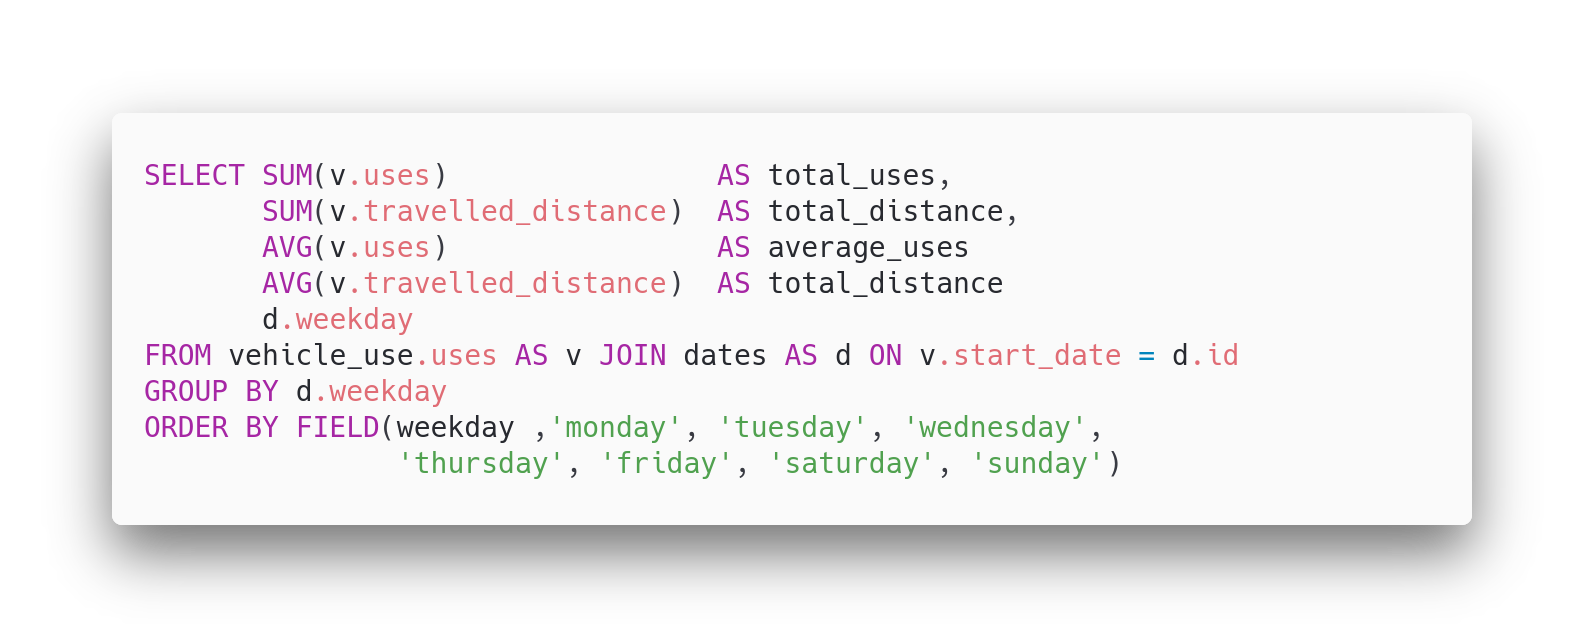
\includegraphics[width=\textwidth]{images/query1}                                                                                                                                   
\label{fig:query1}                                                                                                                                                           
\end{figure}

\iffalse
SELECT SUM(v.uses)                AS total_uses, 
	   SUM(v.travelled_distance)  AS total_distance, 
       AVG(v.uses)                AS average_uses,
       AVG(v.travelled_distance)  AS total_distance,
       d.weekday
FROM vehicle_use.uses AS v JOIN dates AS d ON v.start_date = d.id
GROUP BY d.weekday
ORDER BY FIELD(weekday ,'monday', 'tuesday', 'wednesday',
			   'thursday', 'friday', 'saturday', 'sunday')
\fi


\section{Utilizzo per livelli di pioggia mese per mese}
\begin{figure}[H]                                                                                                                                                            
\centering                                                                                                                                                                   
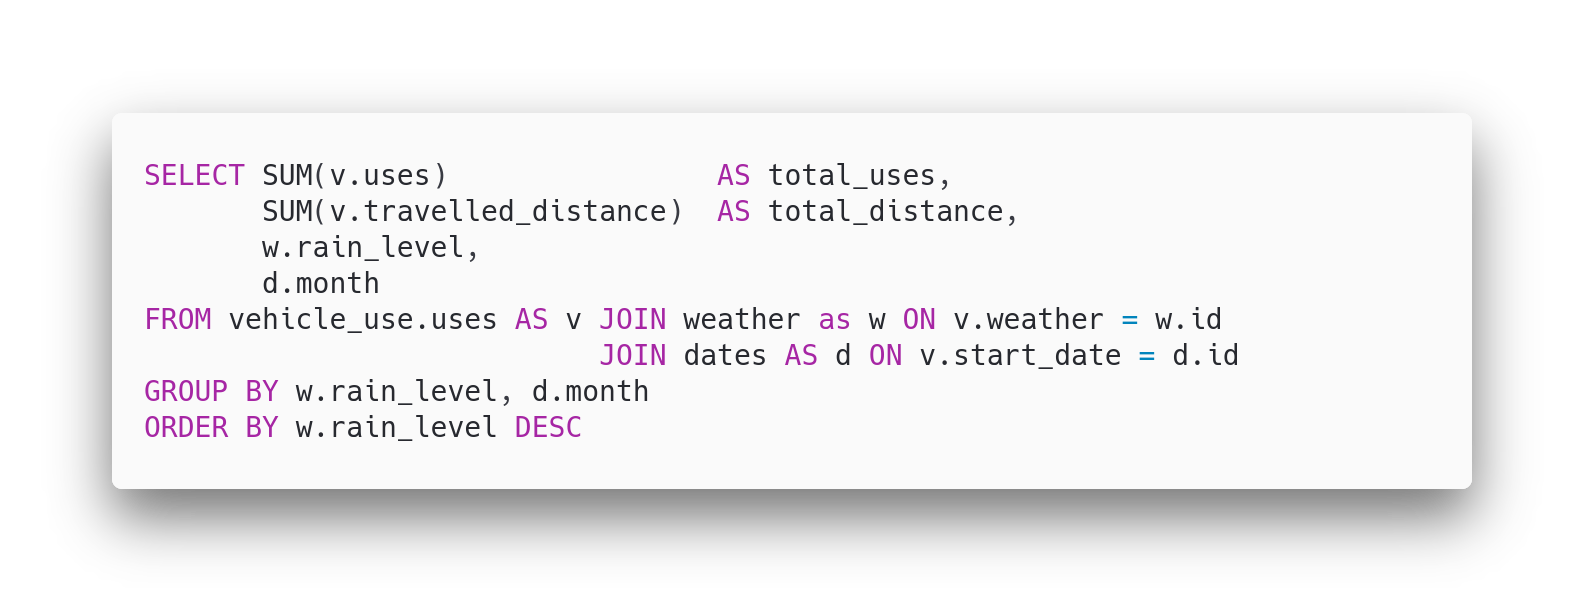
\includegraphics[width=\textwidth]{images/query2}                                                                                                                                   
\label{fig:query2}                                                                                                                                                           
\end{figure}
\iffalse
SELECT SUM(v.uses)                AS total_uses, 
	   SUM(v.travelled_distance)  AS total_distance,
       w.rain_level,
       d.month
FROM vehicle_use.uses AS v JOIN weather as w ON v.weather = w.id
                           JOIN dates AS d ON v.start_date = d.id
GROUP BY w.rain_level, d.month
ORDER BY w.rain_level DESC
\fi


\section{Confronto degli utilizzi durante uno sciopero per fascia oraria}
\begin{figure}[H]                                                                                                                                                            
\centering                                                                                                                                                                   
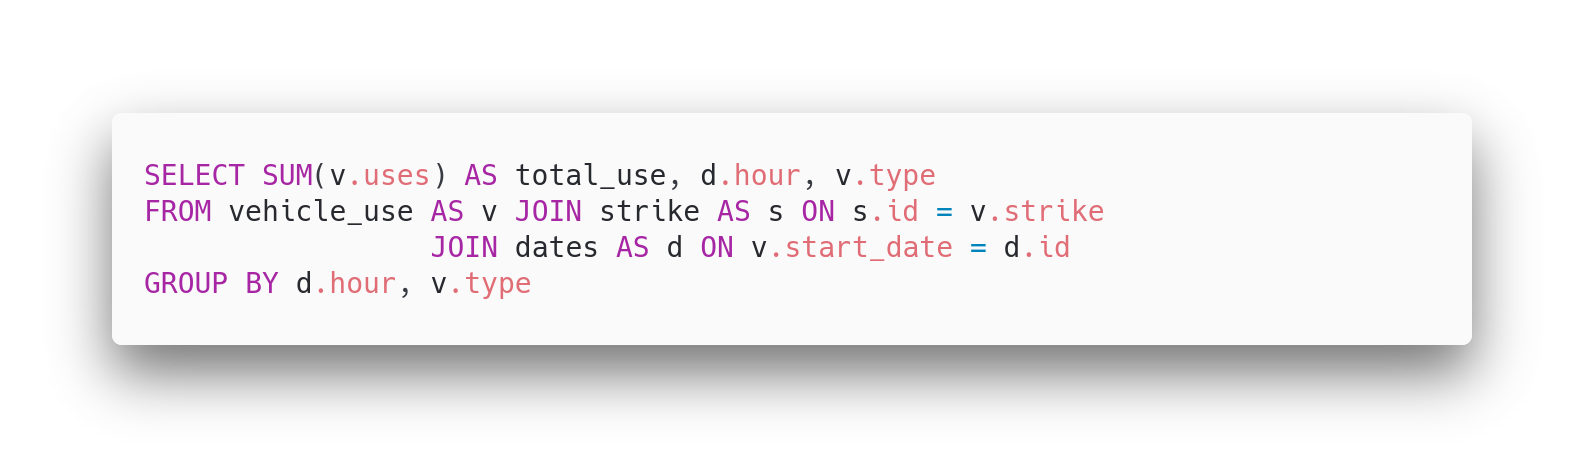
\includegraphics[width=\textwidth]{images/query3}                                                                                                                                   
\label{fig:query3}                                                                                                                                                           
\end{figure}
\iffalse
SELECT SUM(v.uses) AS total_use, d.hour
FROM vehicle_use AS v JOIN strike AS s ON s.id = v.strike
				 JOIN dates AS d ON v.start_date = d.id
GROUP BY d.hour
\fi


\section{Delta utilizzi al variare delle temperature a dipendere della presenza di scioperi}
\begin{figure}[H]                                                                                                                                                            
\centering                                                                                                                                                                   
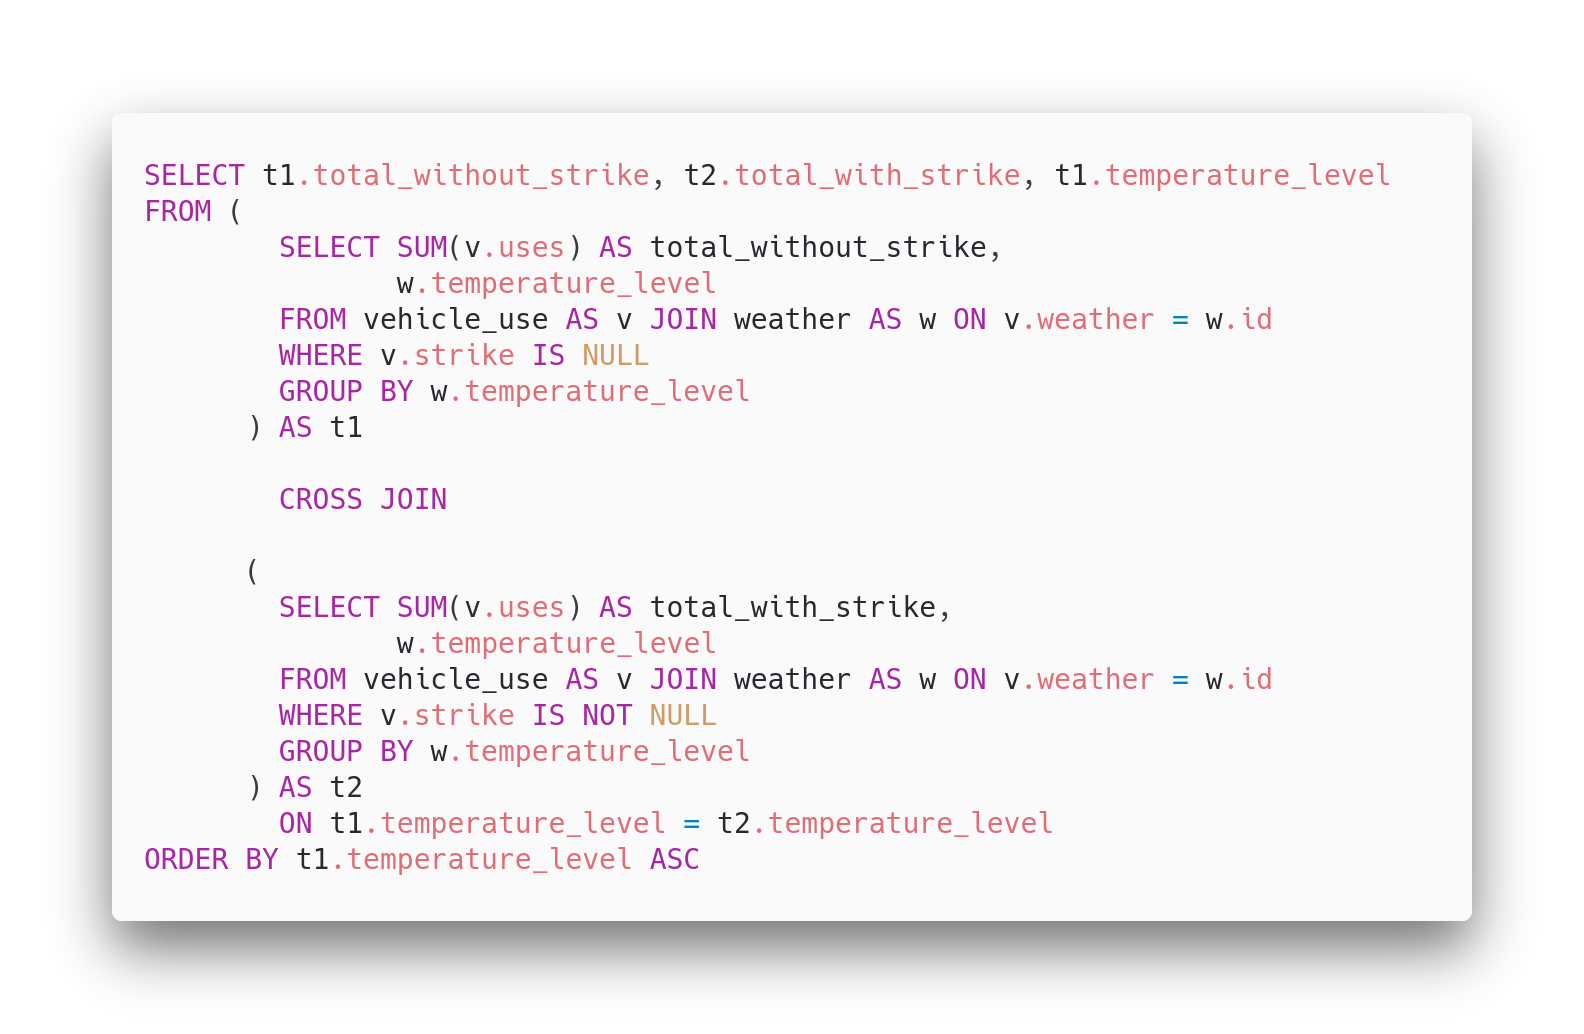
\includegraphics[width=\textwidth]{images/query4}                                                                                                                                   
\label{fig:query4}                                                                                                                                                           
\end{figure}
\iffalse
SELECT t1.total_without_strike, t2.total_with_strike, t1.temperature_level
FROM (
		SELECT SUM(v.uses) AS total_without_strike, 
  			   w.temperature_level
  		FROM vehicle_use AS v JOIN weather AS w ON v.weather = w.id
  		WHERE v.strike IS NULL
  		GROUP BY w.temperature_level
      ) AS t1 
      	
        CROSS JOIN
      
      (
        SELECT SUM(v.uses) AS total_with_strike, 
               w.temperature_level
  		FROM vehicle_use AS v JOIN weather AS w ON v.weather = w.id
        WHERE v.strike IS NOT NULL
  		GROUP BY w.temperature_level
      ) AS t2
        ON t1.temperature_level = t2.temperature_level
ORDER BY t1.temperature_level ASC
\fi


\section{Numero di utilizzi durante uno sciopero nelle ore di punta}
\begin{figure}[H]                                                                                                                                                            
\centering                                                                                                                                                                   
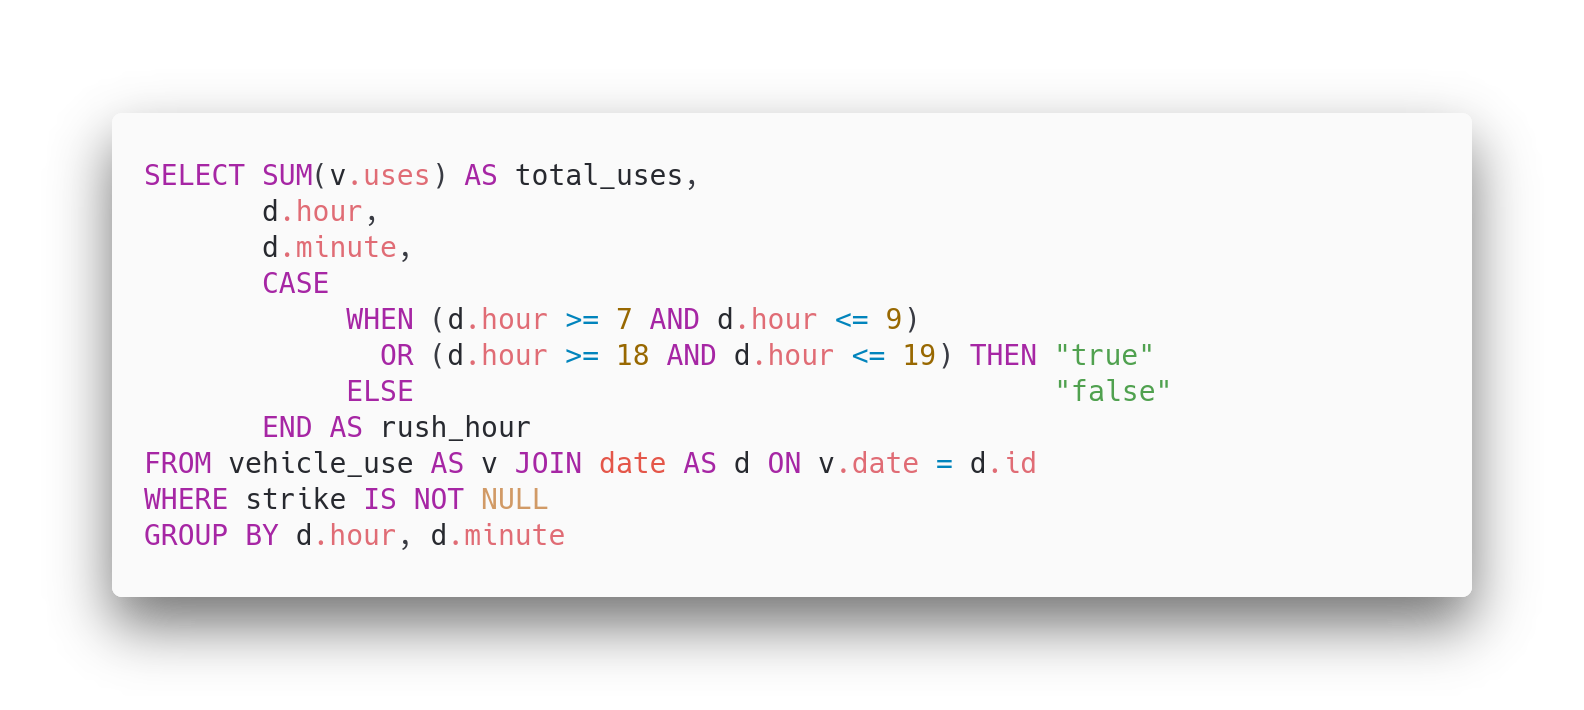
\includegraphics[width=\textwidth]{images/query5}                                                                                                                                   
\label{fig:query5}                                                                                                                                                           
\end{figure}
\iffalse
SELECT SUM(v.uses) AS total_uses, 
       d.hour,
       d.minute,
       CASE 
       		WHEN (d.hour >= 7 AND d.hour <= 9)   
           	  OR (d.hour >= 18 AND d.hour <= 19) THEN "true"
       		ELSE 								      "false"
       END AS rush_hour
FROM vehicle_use AS v JOIN date AS d ON v.date = d.id
WHERE strike IS NOT NULL
GROUP BY d.hour, d.minute
\fi


\section{Numero di utilizzi durante diverse fasce orarie}
\begin{figure}[H]                                                                                                                                                            
\centering                                                                                                                                                                   
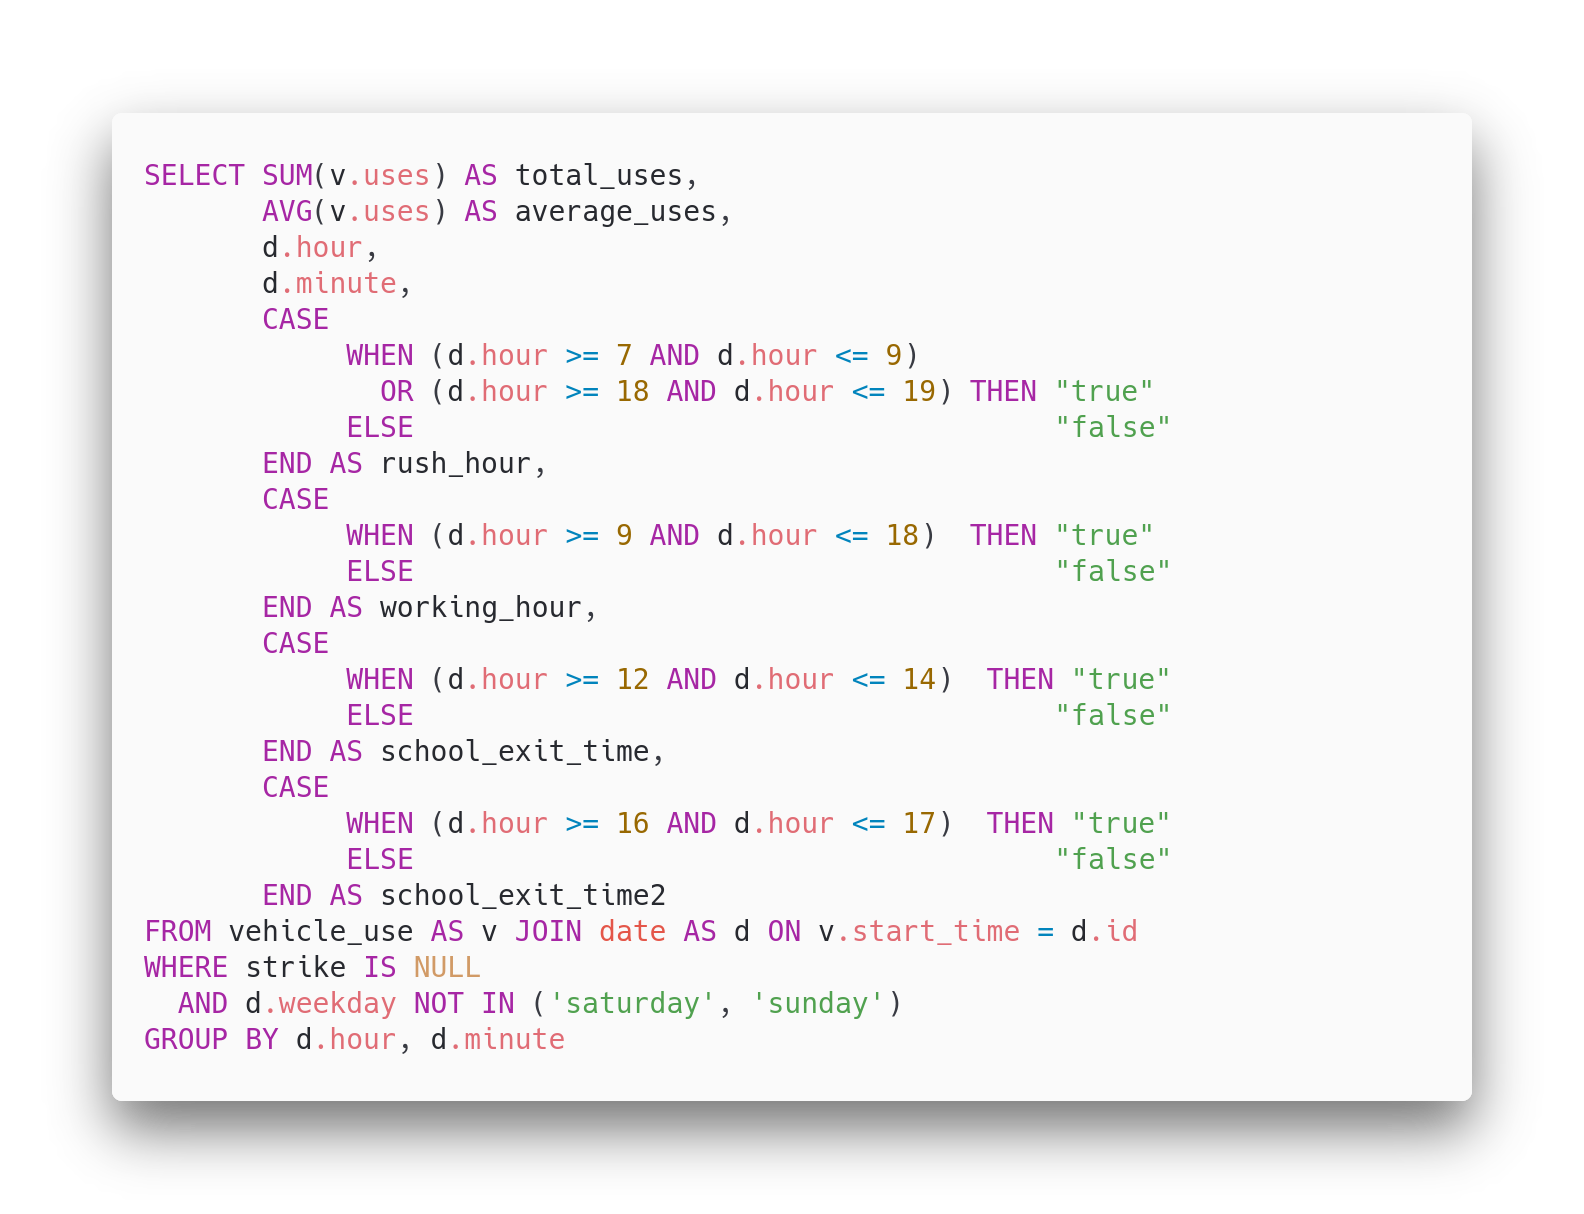
\includegraphics[width=\textwidth]{images/query6}                                                                                                                                   
\label{fig:query6}                                                                                                                                                           
\end{figure}
\iffalse
SELECT SUM(v.uses) AS total_uses,
	   AVG(v.uses) AS average_uses,
       d.hour,
       d.minute,
       CASE 
       		WHEN (d.hour >= 7 AND d.hour <= 9)   
           	  OR (d.hour >= 18 AND d.hour <= 19) THEN "true"
       		ELSE 								      "false"
       END AS rush_hour,
       CASE 
       		WHEN (d.hour >= 9 AND d.hour <= 18)  THEN "true"
       		ELSE 								      "false"
       END AS working_hour,
       CASE 
       		WHEN (d.hour >= 12 AND d.hour <= 14)  THEN "true"
       		ELSE 								      "false"
       END AS school_exit_time,
       CASE 
       		WHEN (d.hour >= 16 AND d.hour <= 17)  THEN "true"
       		ELSE 								      "false"
       END AS school_exit_time2
FROM vehicle_use AS v JOIN dates AS d ON v.date = d.id
WHERE strike IS NULL
  AND d.weekday NOT IN ('saturday', 'sunday')
GROUP BY d.hour, d.minute
\fi